\documentclass[UTF8,10pt,a4paper,fontset=fandol]{ctexart}
\usepackage[margin=19mm]{geometry}
\usepackage{graphicx,booktabs,tabularx,hyperref,float}
\hypersetup{hidelinks}
\setlength{\parindent}{2em}
\setlength{\parskip}{3pt}
\setlength{\textfloatsep}{10pt}
\title{因子流动性测试报告}\date{}\author{}
\begin{document}
{\Large\bfseries 因子流动性测试报告}\par
本次输入因子：F000001收益率因子，测试期为2024-01-02至2024-08-30。目前已完成49个资金账户的全期回放，并核对了现金、持仓和净值。其中，0个资金档完成了全部当日交易计划，49个未达到这一要求，0个仍待核实。目前还没有找到满足这一标准的资金档，下面结合未完成计划说明原因。运行记录中另有1个资金档标记为计算中，记录所载已完成162个交易日；本报告未核实这些进程当前是否运行。

\begin{table}[H]\centering\small
\begin{tabular}{llllr}\toprule
回看期 & 情景 & 最大已测通过 & 更高未通过档 & 已测档数\\\midrule
N20 & 常规 & 尚无 & 尚无 & 5 \\
N20 & 扫板 & 尚无 & 尚无 & 4 \\
N61 & 常规 & 尚无 & 尚无 & 5 \\
N61 & 扫板 & 尚无 & 尚无 & 5 \\
N121 & 常规 & 尚无 & 尚无 & 5 \\
N121 & 扫板 & 尚无 & 尚无 & 5 \\
N241 & 常规 & 尚无 & 尚无 & 5 \\
N241 & 扫板 & 尚无 & 尚无 & 5 \\
N481 & 常规 & 尚无 & 尚无 & 5 \\
N481 & 扫板 & 尚无 & 尚无 & 5 \\
\bottomrule\end{tabular}
\end{table}
表中的“最大已测通过”是本次窗口和执行条件下，已经逐档验证通过的最大资金。未测区间和待核实账户仍需继续检查；“尚无”表示还没有找到通过档，而不是把容量记为零。

\begin{table}[H]\centering\small\begin{tabular}{llllrl}\toprule N & 情景 & 当前资金 & 已完成日期 & 交易日 & 保存的状态\\\midrule N20 & 常规 & 30亿元 & 2024-04-15 & 67/162 & 保存进度待核 \\
N20 & 扫板 & 10亿元 & 2024-08-30 & 162/162 & 记录为计算中 \\
N61 & 常规 & 30亿元 & 2024-01-10 & 7/162 & 保存进度待核 \\
N61 & 扫板 & 30亿元 & 2024-01-10 & 7/162 & 保存进度待核 \\
N121 & 常规 & 30亿元 & 2024-02-07 & 27/162 & 保存进度待核 \\
N121 & 扫板 & 30亿元 & 2024-02-07 & 27/162 & 保存进度待核 \\
N241 & 常规 & 30亿元 & 2024-04-19 & 71/162 & 保存进度待核 \\
N241 & 扫板 & 30亿元 & 2024-04-19 & 71/162 & 保存进度待核 \\
N481 & 常规 & 30亿元 & 2024-04-15 & 67/162 & 保存进度待核 \\
N481 & 扫板 & 30亿元 & 2024-04-15 & 67/162 & 保存进度待核 \\\bottomrule\end{tabular}\end{table}

\section*{因子和实验设置}
使用过去N个交易日复权价格变化的原始信号，经原批次预处理后取G1并等权配置。不同N只改变原回看期版本，不重选参数。

N表示因子的回看期，H表示调仓间隔，两者都按交易日计算。



各资金档沿用同一套选股和调仓规则，每次调仓根据账户净值把目标权重换成目标股数，再与实际持仓比较，得到需要买卖的数量。账户中的现金、持仓和权益连续保留到下一交易日。当前程序按2024年沪深市场规则，采用09:35决策时点和约定的执行窗口。

本报告账户的金融规则版本为g1-0935-event-updates-20261027-v1。本报告保存账户沿用参考价年龄上限规则：参考价必须严格早于09:35、属于当日早盘且年龄不超过30秒。因此正常静默也可能产生年龄超限的待定量目标；这属于该账户的模型时效限制，不证明源数据损坏。重新生成报告没有按新的事件状态参考规则重算这些账户。

订单发出后，经过设定的报单延迟，才在后续合格快照上模拟成交。当时只能成交一部分，就先记下这部分成交并保留余单。所有买卖共用同一个现金账户：买单预留的资金不能再分给其他订单，卖单实际成交后才增加可用现金。未完成的目标和后续调仓都从这一实际账户状态继续计算。

本次从1000万元开始，逐档增加资金，测试上限为100亿元。每档都单独回放账户，并在已测通过与未通过的资金档之间继续细化。

常规情景的成交量参与率为10\%。指令生效后，程序根据后续合格快照中观察到的新增成交量，逐步释放该股票的成交额度。同一股票的多笔订单共同使用这份额度，盘口中可见的对手方数量也会限制成交。此外，策略在该股的累计成交金额最多占截至当时市场已公布累计成交额的10\%。

扫板是另一种执行情景：距涨跌停幅度差1个百分点时触发，即上涨9\%／19\%时买入，下跌9\%／19\%时卖出，对应10\%／20\%涨跌幅制度。触发后，假设后续观察到的市场新增成交量全部可供本策略使用，买入按官方涨停价、卖出按官方跌停价记账。现金和可卖量仍受账户约束。原扫板基线采用乐观成交假设，没有额外冲击成本；启用冲击的情景另列，均未模拟真实排队竞争。

容量的通过条件是：测试期内，每笔计划交易都在计划当天100\%完成。单笔完成率等于当日成交量除以计划量；即使只剩一笔小额余单，当天也没有达到全部完成的要求。停牌、涨跌停、现金或数量限制仍计入这一检查，并在后文分别解释。资料不足、计划量尚不明确的目标保留待核。

报告同时展示模型收益和按金额衡量的完成情况。模型收益等于期末净值除以初始资金再减一。基线佣金税费为0；额外模型冲击单独列示，启用时在成交前进入现金和数量计算。盘口价差、跨档及扫板价格成本已包含在成交金额中，不再重复扣除。金额完成率用计划时的参考价把买卖股数换算成金额，买入和卖出都按正数合计；图中展示完成情况最差的一天。容量是否通过仍按逐笔100\%判断。

\section*{资金规模与收益、成交}
\begin{figure}[H]\centering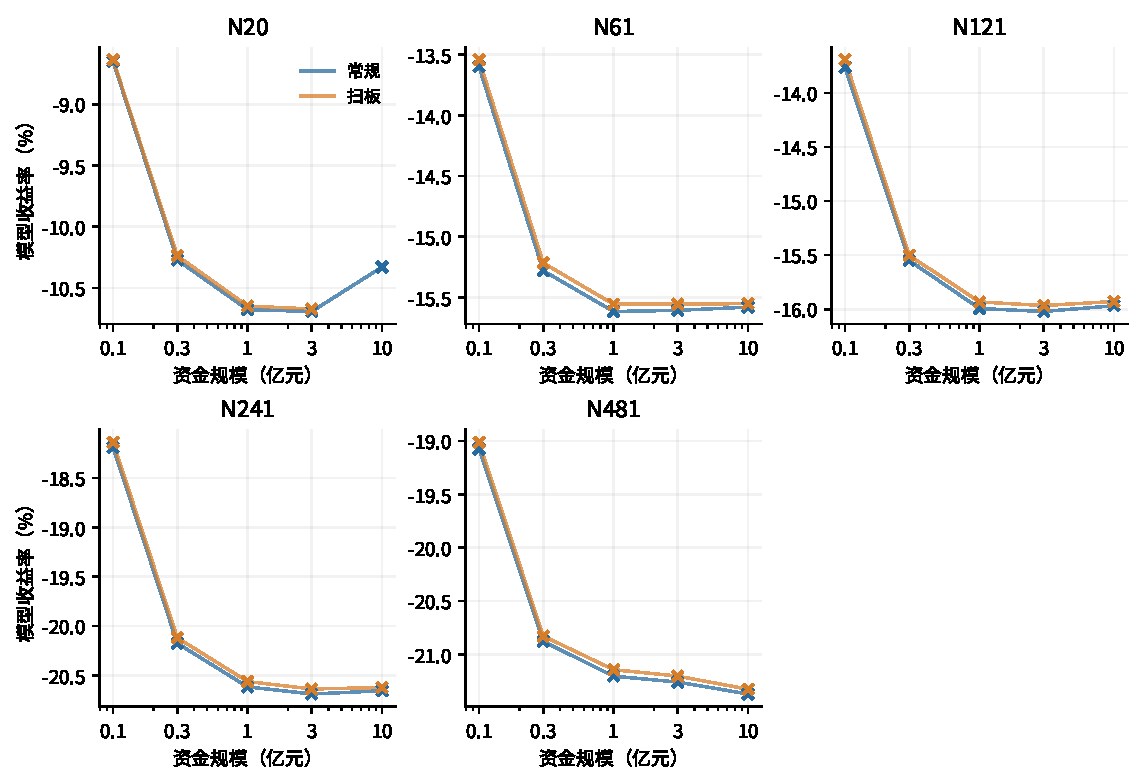
\includegraphics[width=.82\linewidth]{figures/capital_return.pdf}
\caption{不同资金规模下的全期模型收益。点表示已完成回放并核账的资金档，连线不代表未测区间通过；冲击情景使用扣除额外模型成本后的账户净值。}\end{figure}
\begin{figure}[H]\centering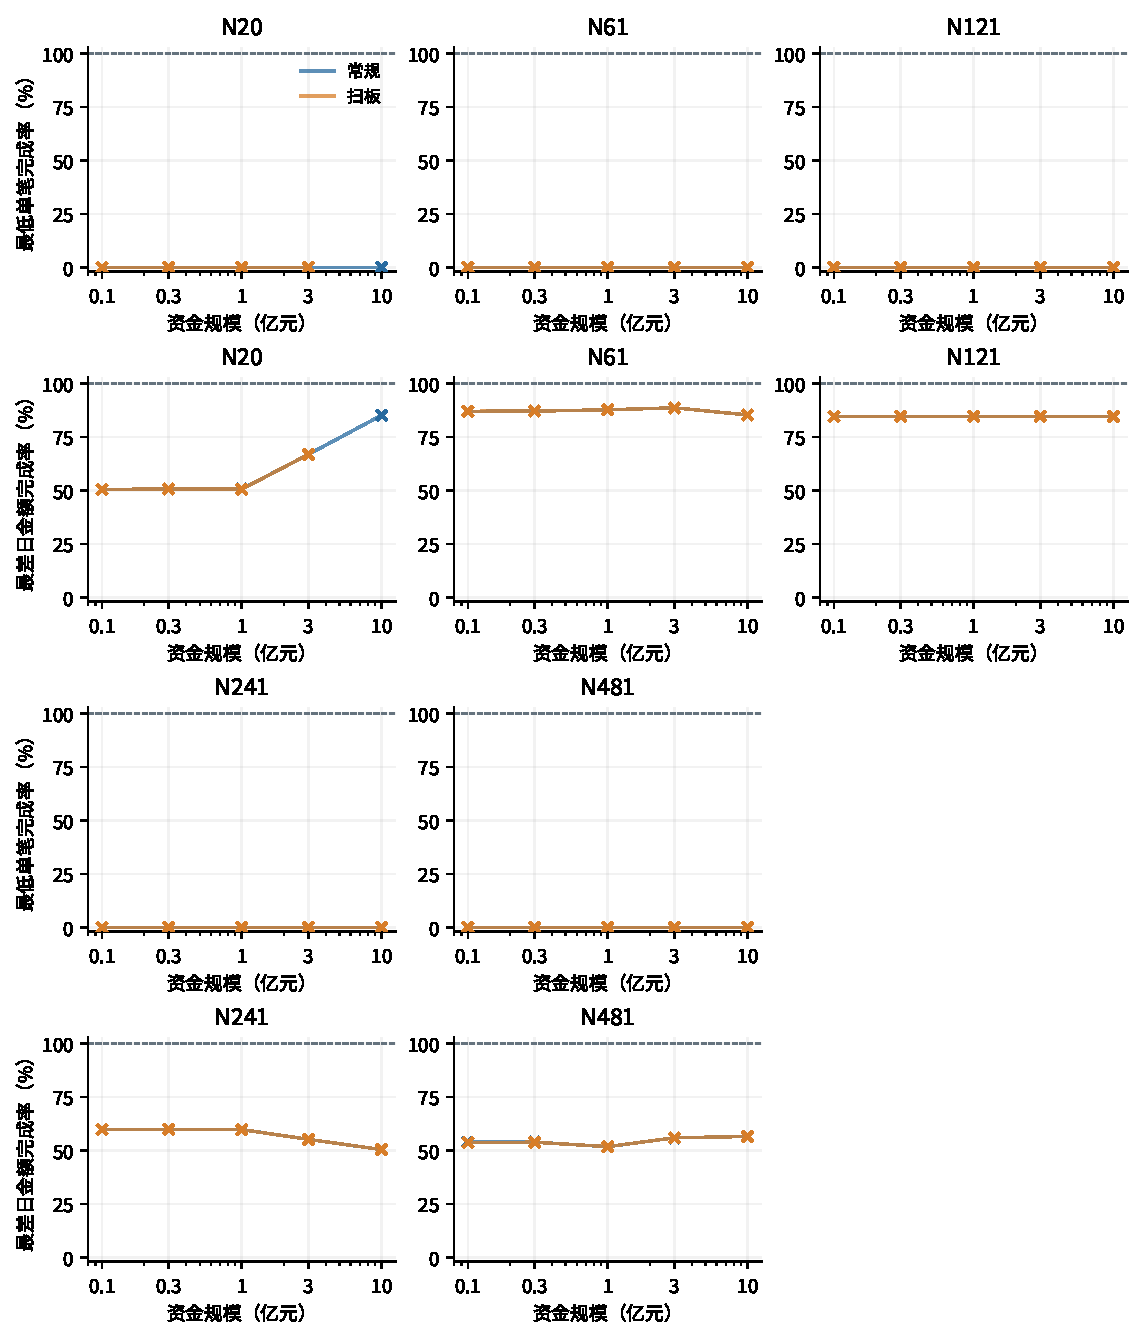
\includegraphics[width=\linewidth]{figures/capital_completion.pdf}
\caption{资金与最低单笔完成率、最差交易日金额完成率。颜色区分执行情景；圆点通过、叉号未通过、三角待核实。}\end{figure}
\section*{原计划完成时间}以原计划日的固定正数量需求为分母，30／60分钟均为交易分钟，扣除午休。跨日重试不新增计划，也不改写原日结果。未完成计划和缺时间证据的计划保留在分母；待定量目标另列在随附表。下表列各组最低已测资金，全部资金及已完成计划耗时分位数见图源表。\begin{table}[H]\centering\scriptsize\begin{tabular}{lllrrrrr}\toprule N & 情景 & 资金 & 正计划 & 30分全成 & 60分全成 & 当日未成 & 时间待核\\\midrule N121 & 常规 & 1000万元 & 7991 & 6732 & 6770 & 1183 & 0 \\
N121 & 扫板 & 1000万元 & 7983 & 6741 & 6778 & 1167 & 0 \\
N20 & 扫板 & 1000万元 & 11835 & 10599 & 10705 & 1040 & 0 \\
N20 & 常规 & 1000万元 & 11836 & 10586 & 10694 & 1051 & 0 \\
N241 & 扫板 & 1000万元 & 6924 & 5586 & 5626 & 1270 & 0 \\
N481 & 常规 & 1000万元 & 6282 & 5137 & 5165 & 1084 & 0 \\
N241 & 常规 & 1000万元 & 6929 & 5583 & 5625 & 1276 & 0 \\
N481 & 扫板 & 1000万元 & 6282 & 5148 & 5175 & 1074 & 0 \\
N61 & 常规 & 1000万元 & 9219 & 7977 & 8046 & 1115 & 0 \\
N61 & 扫板 & 1000万元 & 9221 & 7998 & 8067 & 1097 & 0 \\\bottomrule\end{tabular}\end{table}
\section*{哪些交易没有完成}
\begin{table}[H]\centering\scriptsize\begin{tabular}{lllllrrr}\toprule 证券 & 日期 & N & 情景 & 资金 & 计划量 & 成交量 & 余量\\\midrule 证券1 & 05-17 & N20 & 常规 & 1000万元 & 104 & 0 & 104 \\
证券2 & 05-17 & N20 & 常规 & 1000万元 & 191 & 0 & 191 \\
证券1 & 05-17 & N20 & 扫板 & 1000万元 & 104 & 0 & 104 \\
证券2 & 05-17 & N20 & 扫板 & 1000万元 & 191 & 0 & 191 \\
证券3 & 04-16 & N61 & 常规 & 1000万元 & 2,300 & 0 & 2,300 \\
证券4 & 06-17 & N61 & 常规 & 1000万元 & 11,499 & 0 & 11,499 \\
证券5 & 04-16 & N61 & 扫板 & 1000万元 & 5,100 & 0 & 5,100 \\
证券6 & 03-15 & N61 & 扫板 & 1000万元 & 136 & 0 & 136 \\\bottomrule\end{tabular}\end{table}\begin{table}[H]\centering\scriptsize\begin{tabular}{llrrrrr}\toprule 证券 & 日期 & 前20日均额(万) & 当日额(万) & 当日/均额 & 扫板 & 扫板成交量\\\midrule 证券1 & 05-17 & 待核 & 2,757.12 & 待核 & 否 & 0 \\
证券2 & 05-17 & 待核 & 6,484.58 & 待核 & 否 & 0 \\
证券1 & 05-17 & 待核 & 2,757.12 & 待核 & 否 & 0 \\
证券2 & 05-17 & 待核 & 6,484.58 & 待核 & 否 & 0 \\
证券3 & 04-16 & 8,541.33 & 309.4 & 0.04 & 否 & 0 \\
证券4 & 06-17 & 11,511.32 & 11,866.5 & 1.03 & 否 & 0 \\
证券5 & 04-16 & 待核 & 43.75 & 待核 & 否 & 0 \\
证券6 & 03-15 & 待核 & 172,962.95 & 待核 & 否 & 0 \\\bottomrule\end{tabular}\end{table}\begin{figure}[H]\centering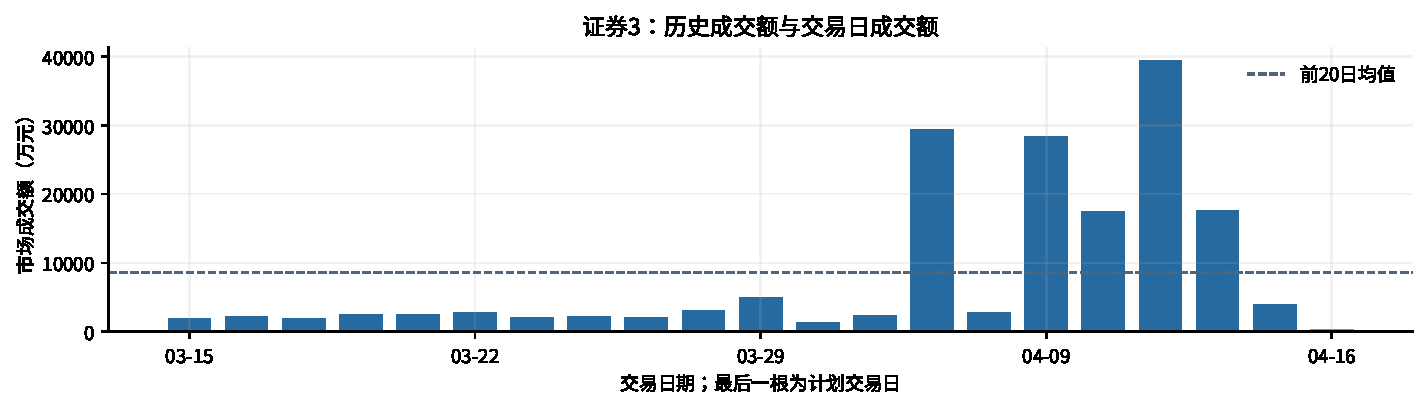
\includegraphics[width=\linewidth]{figures/turnover_case.pdf}\caption{同一证券在此前20个交易日和计划交易日的成交额，虚线为前20日均值。}\end{figure}图表用证券编号展示，实际股票代码和逐笔明细保存在私有结果目录。

前20日均成交额用来观察股票平时的交易活跃度，当日成交额则帮助判断计划交易日是否明显放量或缩量。均值取此前20个官方交易日，已确认零成交的日期也计入；历史资料不足时留空。当日成交额用于事后解释，盘中下单不会提前知道这个数。是否因历史放量而入选，还需要结合原选股规则判断。

案例1为N481的常规账户，资金10亿元，2024-04-16原计划234300股／份，当日实际成交0，剩余234300。该计划没有已保存的扫板触发证据。\begin{figure}[H]\centering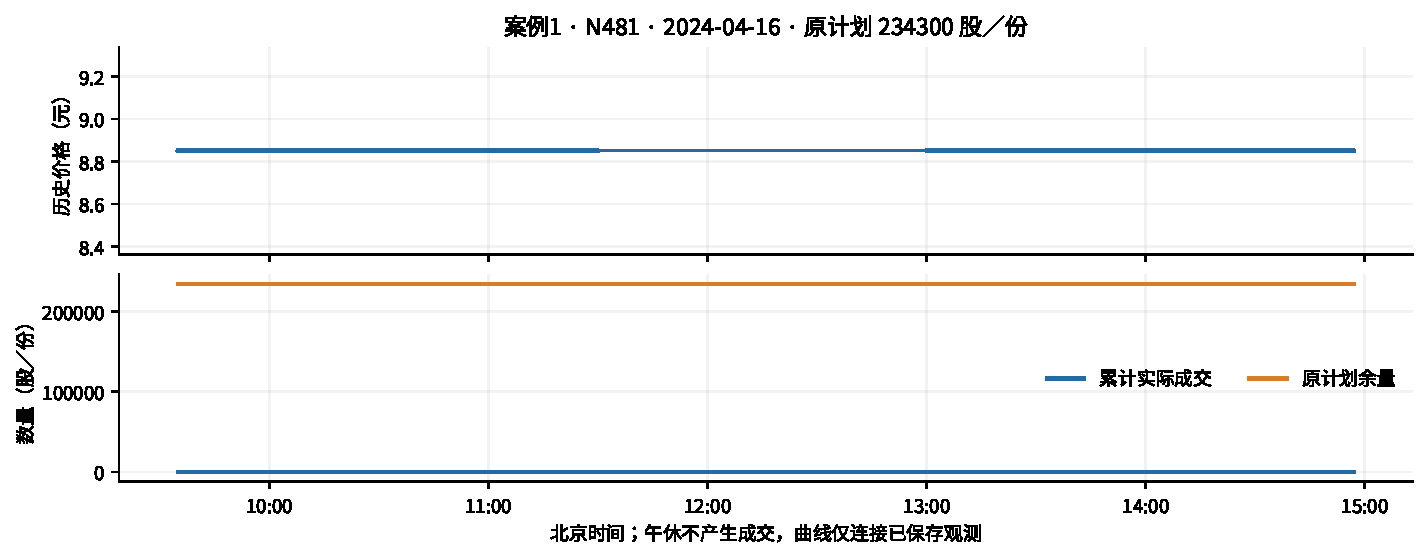
\includegraphics[width=\linewidth]{figures/intraday_1.pdf}\caption{实际历史观测与该账户的原计划执行。不同情景各用自己的计划与账户路径。}\end{figure}案例2为N481的扫板账户，资金10亿元，2024-04-16原计划234300股／份，当日实际成交101700，剩余132600。扫板首次触发于09:35:00。\begin{figure}[H]\centering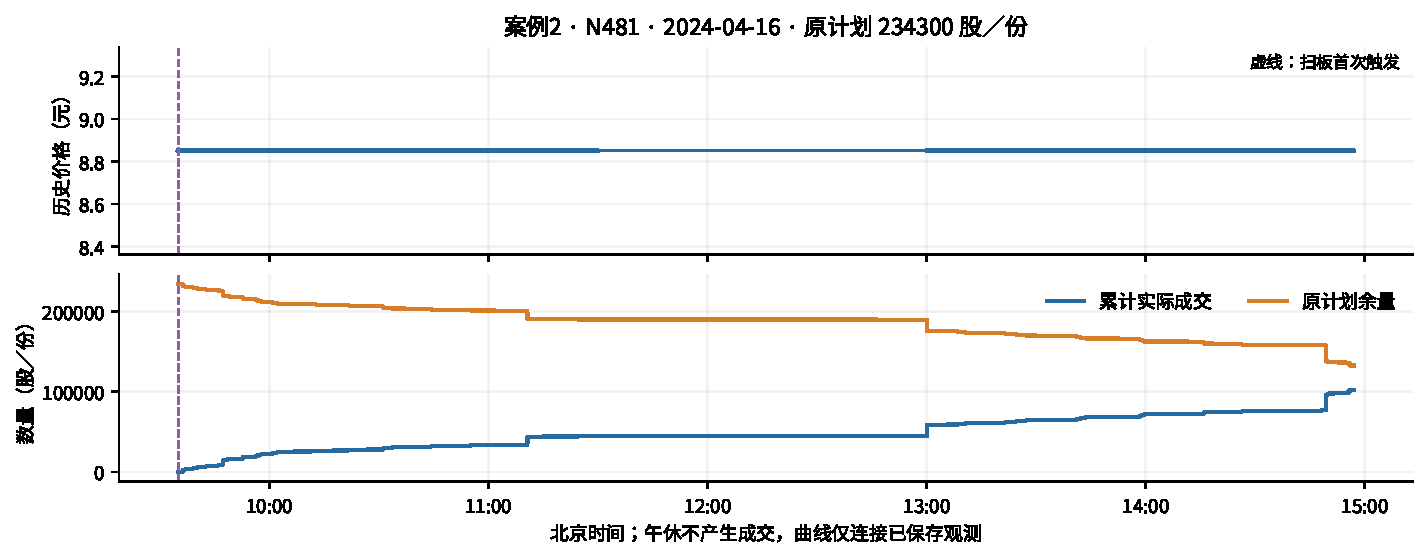
\includegraphics[width=\linewidth]{figures/intraday_2.pdf}\caption{实际历史观测与该账户的原计划执行。不同情景各用自己的计划与账户路径。}\end{figure}案例3为N61的常规账户，资金10亿元，2024-06-17原计划1.1451e+06股／份，当日实际成交0，剩余1.1451e+06。该计划没有已保存的扫板触发证据。\begin{figure}[H]\centering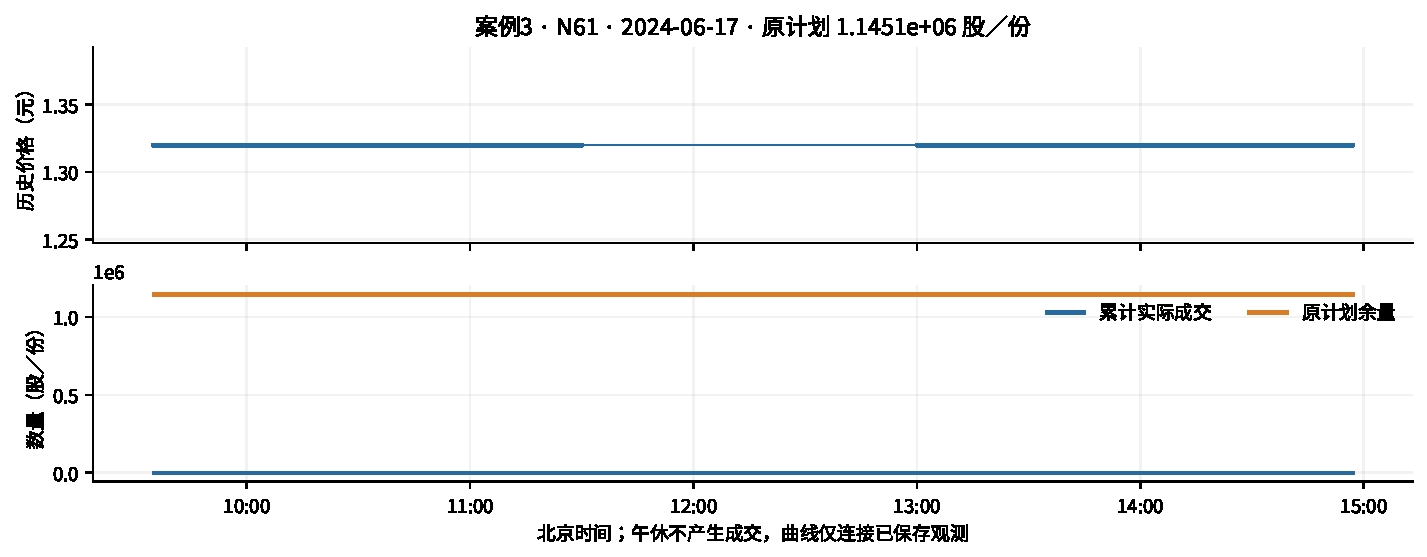
\includegraphics[width=\linewidth]{figures/intraday_3.pdf}\caption{实际历史观测与该账户的原计划执行。不同情景各用自己的计划与账户路径。}\end{figure}

\section*{停牌、涨跌停和其他限制}
下表把交易中遇到的限制分开列出，帮助解释哪些计划没有完成。每笔原始计划只计一次，次日继续交易不会再算一笔新计划。同一计划可能同时遇到几种限制，因此各行数量不能相加。

每个N和情景选一个代表资金档，优先选择资金最小的未完成档。本表使用：N20/常规 1000万元、N20/扫板 1000万元、N61/常规 1000万元、N61/扫板 1000万元、N121/常规 1000万元、N121/扫板 1000万元、N241/常规 1000万元、N241/扫板 1000万元、N481/常规 1000万元、N481/扫板 1000万元。各账户分别计数，同一股票在不同账户中的计划会分别列入。\begin{table}[H]\centering\small\begin{tabular}{lrrr}\toprule 遇到的情况 & 涉及计划 & 仍有未成交量 & 数量待核\\\midrule 有明确停牌记录 & 286 & 0 & 286 \\
停牌记录的日内时段未核实 & 286 & 0 & 286 \\
涨跌停资料或状态待核实 & 140 & 0 & 140 \\
触发扫板假设 & 172 & 23 & 0 \\
初始计划低于最低申报量 & 5342 & 5342 & 0 \\
部分成交后剩余量不能再申报 & 4772 & 4772 & 0 \\
其他数量约束或细分依据不足 & 990 & 990 & 0 \\
记录过现金约束 & 37173 & 3466 & 0 \\
公司行动或权益政策约束 & 3952 & 0 & 3952 \\
参考价或行情资料待核实 & 702 & 593 & 24 \\
未完成条件未归入上述类别 & 238 & 238 & 0 \\\bottomrule\end{tabular}\end{table}

停牌记录涉及286笔计划。其中286笔还缺少明确的起止时间，需要补齐才能判断哪些时段可以交易；另有0笔计划的停牌状态尚待核实。

涨停买入和跌停卖出分别列出。本轮封板记录来自临近日终的有效快照，说明当时价格处于对应限价、对手盘为空。这不证明当天一直封板，也不能据此排除早些时候的成交机会。扫板情景按前文设定单独计算。

数量限制有两种常见情况：目标一开始就小于最低申报量，或部分成交后留下无法再次申报的零头。表中根据计划量、成交量和适用规则区分二者，依据不够的另列。现金不足、可卖数量不足则记录交易过程中曾遇到的限制；条件恢复后，订单仍可继续执行。

分红送转等权益处理与行情资料问题分别列出。缺少参考价、行情或交易状态时，先保留待核状态，补齐资料后再判断成交条件。参考价采用前文所述的本报告账户规则，正常静默本身不证明数据损坏。

\end{document}
